\section{Methods} \label{sec:methods}

\subsection{The Algorithm} \label{sec:algorithm}

We present a modification of Algorithm~\ref{alg:old} where we replace the best path search in line 9 with a more intelligent consolidation step to deal with missing ranks. The main idea of this algorithm is to realize that, as previously stated, once data from a specific rank is no longer included in one organism, it will not be included in any subsequent organisms, meaning that the nodes in the tree corresponding to that rank are no longer useful. So, by building shortcuts around any nodes that were made irrelevant, we can speed up the reconstruction process for all future nodes too.

We detect missing information the same way as in the naive trie algorithm: during iteration, we notice that when a child $c$ of the current node $n$ has a rank $r'$ that is less than the current rank $r$ being processed, we do not have information about that rank. The key insight to the way we manage this is that, in the big picture, we only care about this child if some of its descendants at rank $r$ have the differentia equal to $d$. Also, since every subsequent organism does not contain information at rank $r'$ (due to the sorting), this statement holds throughout the rest of the algorithm.

\begin{figure*}
\begin{minipage}{0.74\linewidth}
\centering
\begin{minipage}{0.32\linewidth}
  \centering
  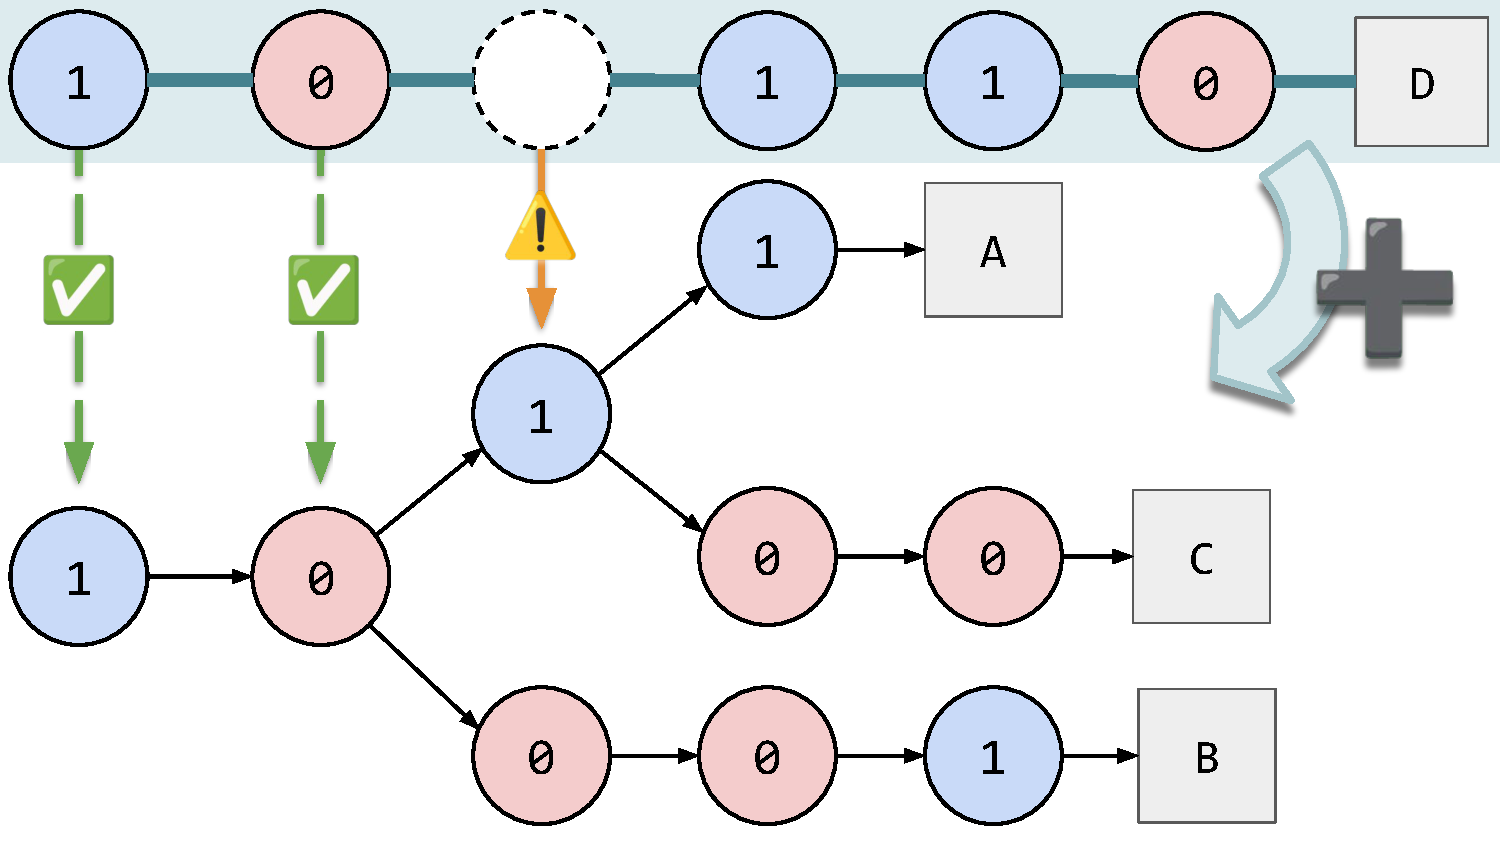
\includegraphics[width=\linewidth]{img/shortcut-algo-diagram-1}
  \subcaption{Preparing to add $D$}
  \label{fig:shortcut-algo-diagram-1}
\end{minipage}
\begin{minipage}{0.32\linewidth}
  \centering
  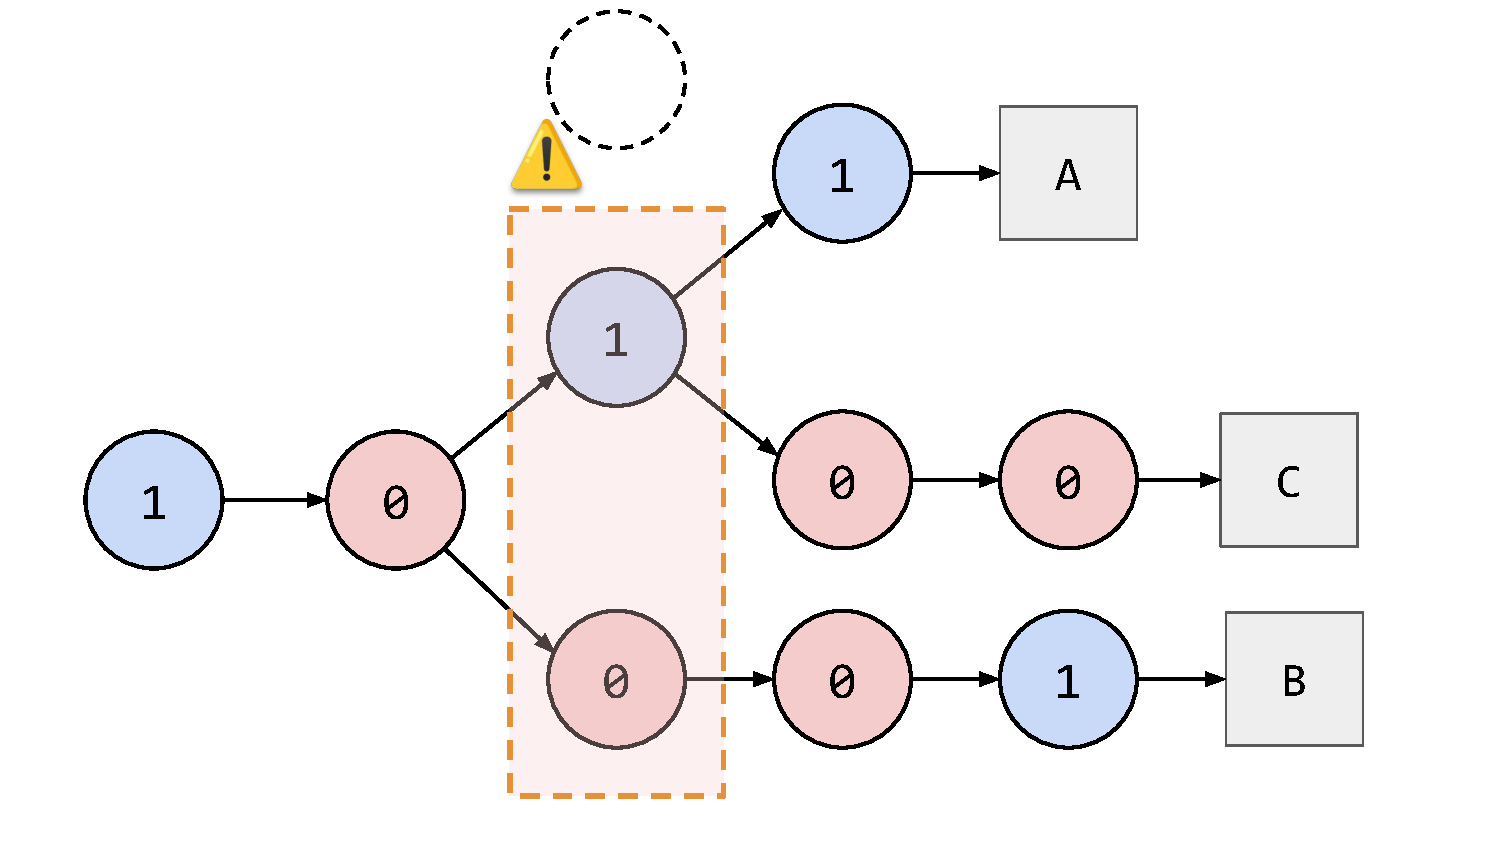
\includegraphics[width=\linewidth]{img/shortcut-algo-diagram-2}
  \subcaption{Encountering dropped marker}
  \label{fig:shortcut-algo-diagram-2}
\end{minipage}
\begin{minipage}{0.32\linewidth}
  \centering
  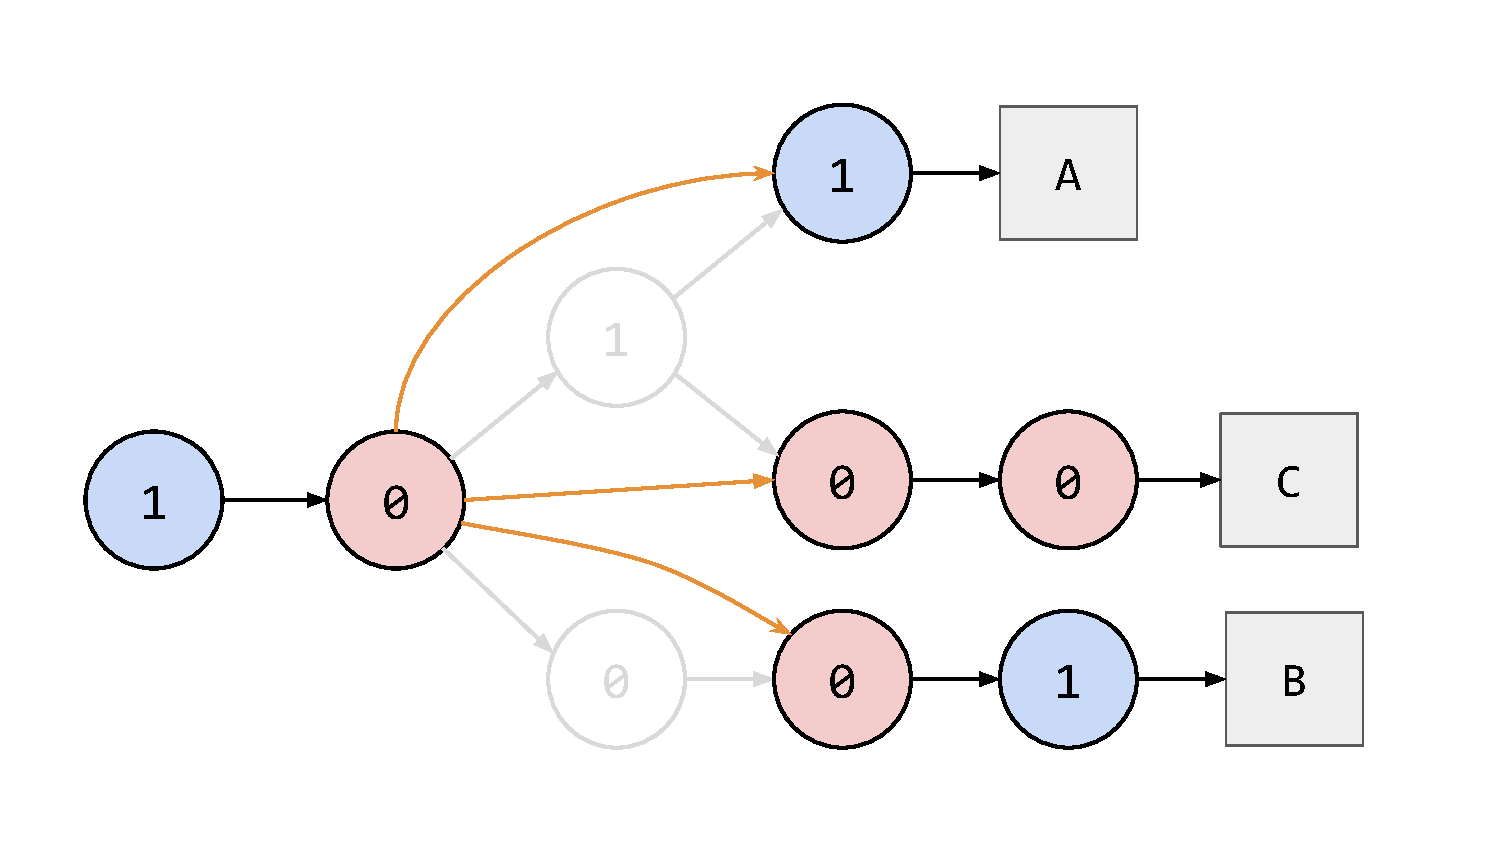
\includegraphics[width=\linewidth]{img/shortcut-algo-diagram-3}
  \subcaption{Building shortcuts}
  \label{fig:shortcut-algo-diagram-3}
\end{minipage}
\begin{minipage}{\linewidth}\par\end{minipage}
\begin{minipage}{0.32\linewidth}
  \centering
  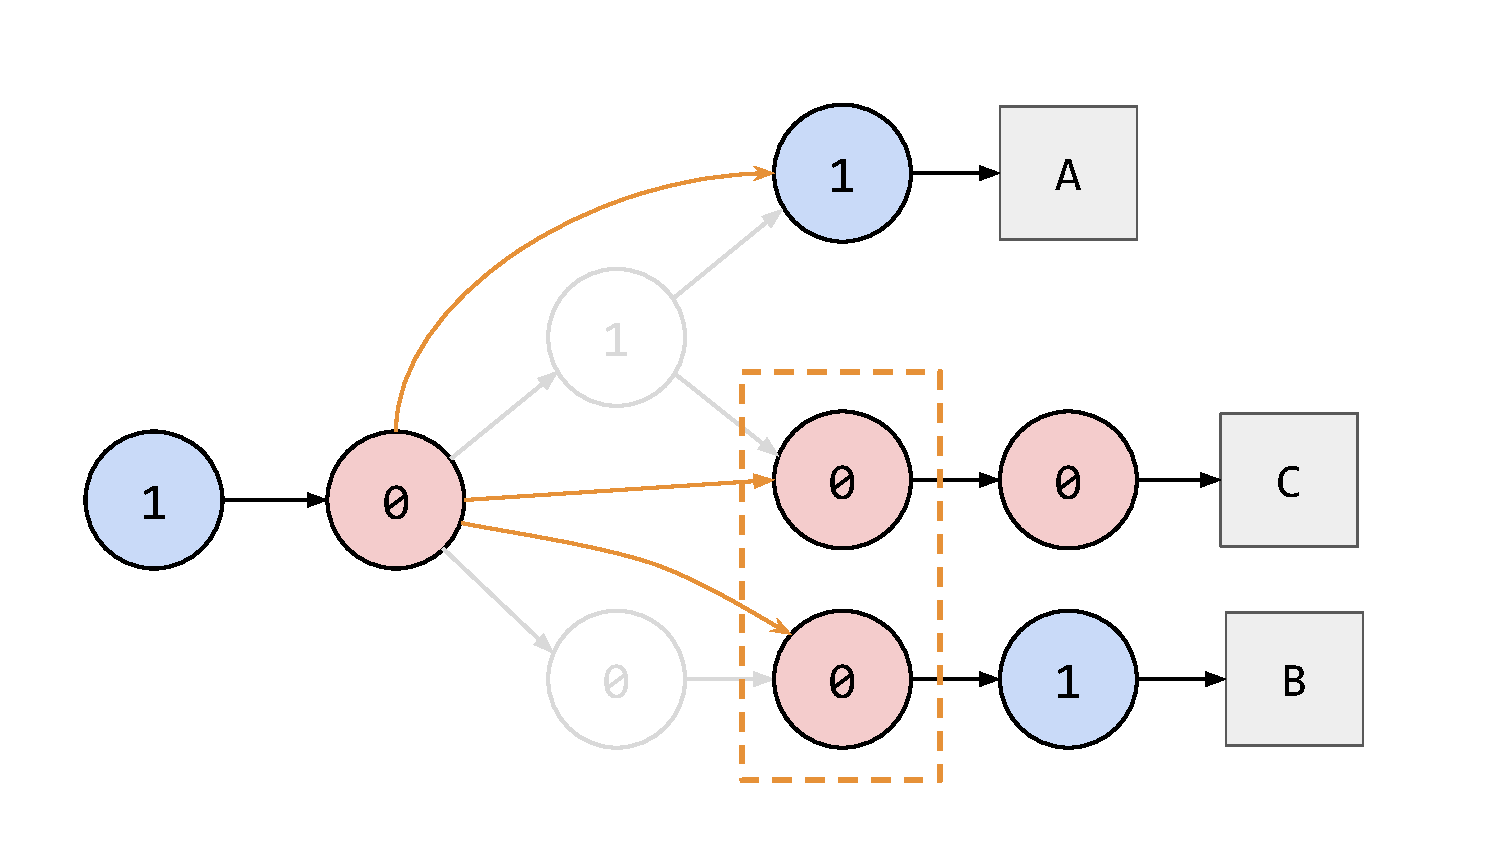
\includegraphics[width=\linewidth]{img/shortcut-algo-diagram-4}
  \subcaption{Indistinguishable nodes}
  \label{fig:shortcut-algo-diagram-4}
\end{minipage}
\begin{minipage}{0.32\linewidth}
  \centering
  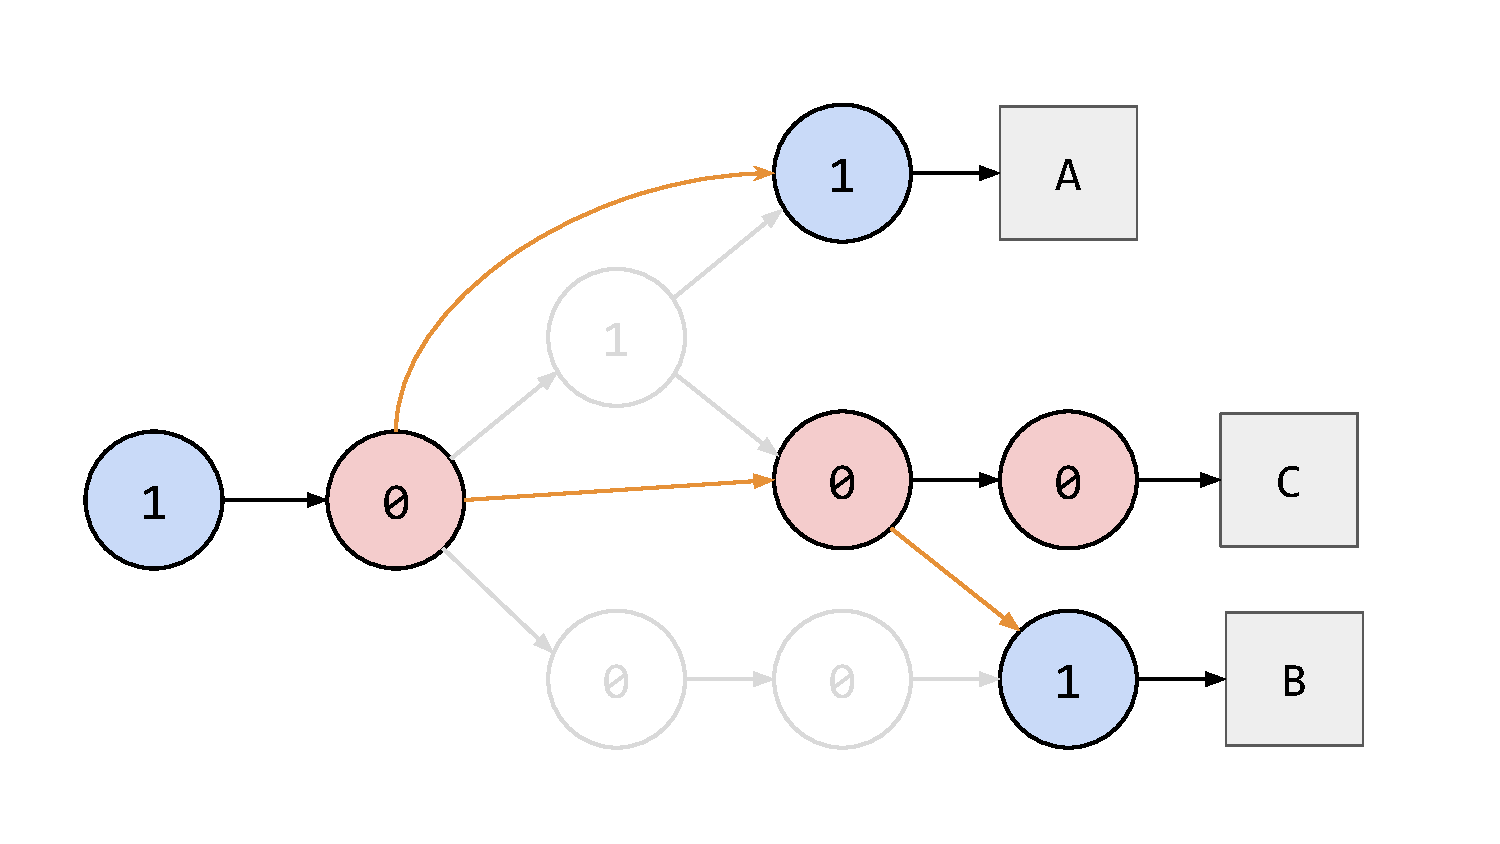
\includegraphics[width=\linewidth]{img/shortcut-algo-diagram-5}
  \subcaption{Collapsing redundant shortcuts}
  \label{fig:shortcut-algo-diagram-5}
\end{minipage}
\begin{minipage}{0.32\linewidth}
  \centering
  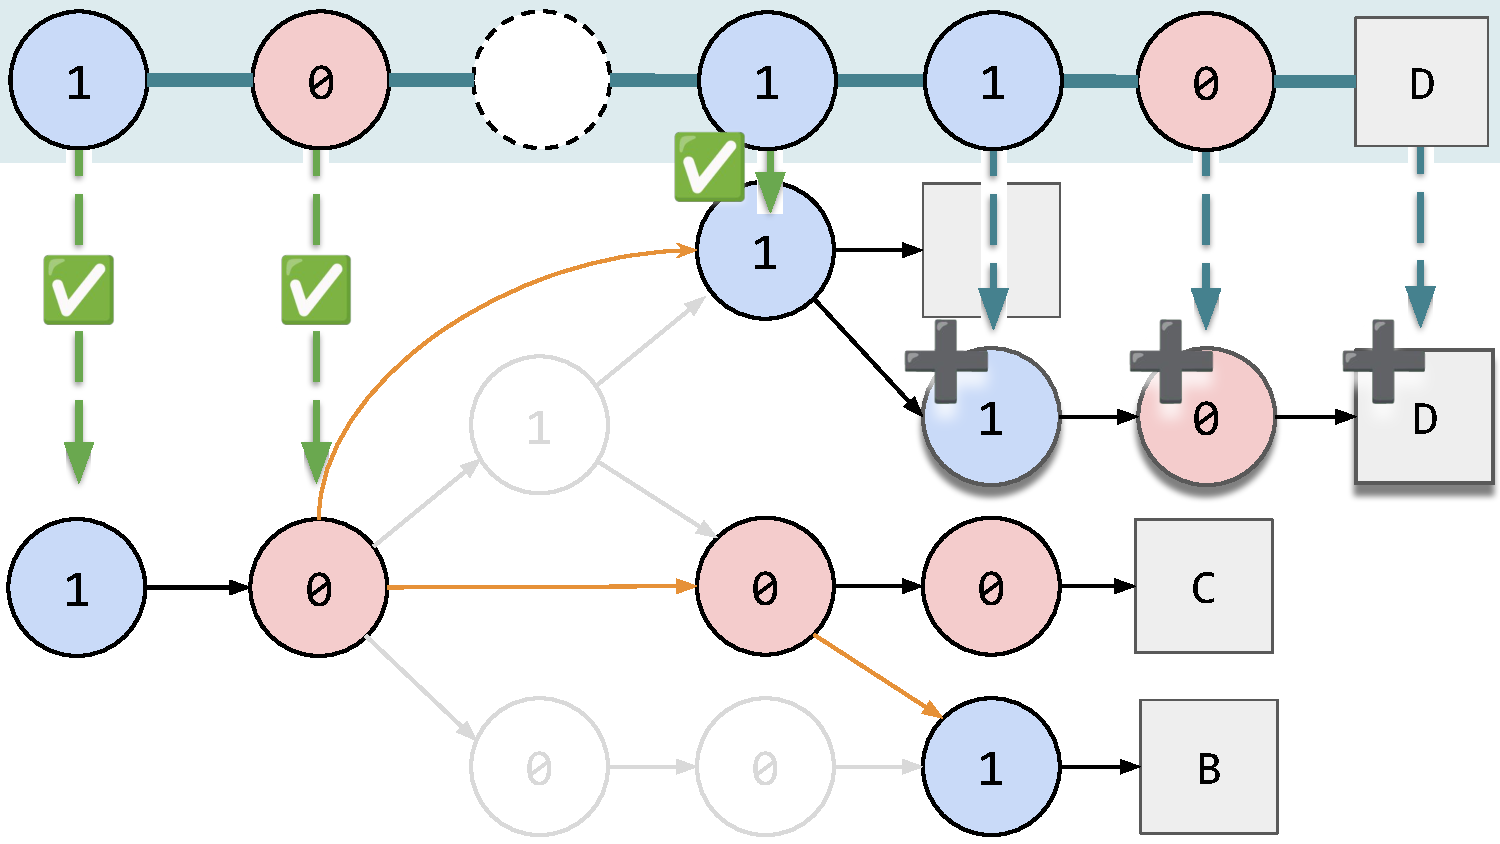
\includegraphics[width=\linewidth]{img/shortcut-algo-diagram-6}
  \subcaption{Organism $D$ added}
  \label{fig:shortcut-algo-diagram-6}
\end{minipage}
\end{minipage}
\begin{minipage}{0.24\linewidth}
\caption{%
\textbf{Trie-consolidation procedure for proposed shortcut algorithm.}
\small
A dropped hereditary marker is encountered while extending trie with genome $D$ (panel \ref{fig:shortcut-algo-diagram-2}).
All subsequent-added genomes will also have dropped markers at this position, so corresponding trie nodes may be bypassed by ``shortcut'' connections (panel \ref{fig:shortcut-algo-diagram-3}).
Note that bypassed trie structure is retained (``grayed-out'' nodes), so corresponding phylogenetic structure remains when reconstruction is finalized.
In a final step, shortcuts leading to identical nodes are further consolidated (panels \ref{fig:shortcut-algo-diagram-4} and \ref{fig:shortcut-algo-diagram-5}).
}
\label{fig:algo-diagram}
\end{minipage}
\vspace{-1.5em}
\end{figure*}


Extending this idea, since we know that any rank between $r'$ and $r$ is meaningless (as they all must have been deleted organism $o$ and any subsequent organisms), we create shortcuts from $n$ that bypass every one of its descendants that have a rank less than $r$. In other words, on every possible path down the tree starting from $n$, we build a shortcut from $n$ to the first node on the tree with a rank at least $r$. For an example of what this looks like, see steps (b) and (c) in Figure~\ref{fig:algo-diagram}. 

However, since some descendants of $n$ may have children with equivalent information, we may end up with shortcuts from $n$ to effectively indistinguishable nodes (with different original parents but the same information). This can be resolved by essentially `merging' the duplicates by choosing one to keep and creating shortcuts from the kept one to the children of the removed one (see steps (d) and (e) in Figure~\ref{fig:algo-diagram}).

Now, adding any organisms that are missing data from the removed level becomes trivial, as the algorithm can use the newly created shortcuts while skipping the missing information that was hidden by the consolidation step. We no longer need to look down branches from $n$ because each child of $n$ now has a rank greater than or equal to $r$. So, there is no longer a concern of missing information when processing $n$ at rank $r$, and these shortcuts are then used to add any subsequent organisms if need be. If, at some point in the algorithm, $r$ itself becomes a rank of missing information, additional shortcuts can be built.

\begin{algorithm}[h]
  \begin{algorithmic}[1]
  \small{
    \Function{ConsolidateTree}{tree $T$, node $n$, rank $r$}
      \State $S \gets \{c \in \operatorname{descendants}(n) : \operatorname{rank}(c) \ge r \land  \operatorname{rank}(\operatorname{parent}(c)) < r\}$ 
      \For{$c$ in $S$} 
        \textsc{BuildShortcut}($T$, $n$, $c$)
      \EndFor
      \For{each subset of duplicate\footnotemark nodes $S' \subseteq S$}
        \State $c^* \gets$ an arbitrary element in $S'$ 
        \For{$c' \in S \setminus \{c^*\}$}
          \For{$c$ in $\operatorname{children}(c)$} 
            \State \textsc{BuildShortcut}($T$, $c^*$, $c$)
          \EndFor
          \State \textsc{RemoveShortcut}($T$, $n$, $c'$)
        \EndFor
      \EndFor 
    \EndFunction
    \Function{BuildShortcut}{tree $T$, node $n$, node $c$}
      \State $\operatorname{edges}(T) \gets \operatorname{edges}(T) \cup \{(n, c)\}$
      \State $\operatorname{edges}(T)[(n, c)]\text{.is\_shortcut} \gets \textsc{True}$
    \EndFunction
    \Function{RemoveShortcut}{tree $T$, node $n$, node $c$}
        \State $\operatorname{edges}(T) \gets \operatorname{edges}(T) \setminus \{(n, c)\}$
    \EndFunction
  }
  \end{algorithmic}
  \caption{\textbf{The consolidation step of the shortcut table algorithm.} \small Builds shortcuts for a given node $n$ and collapses duplicate children caused by those shortcuts. Note that \vspace{-1.5em}}
  \label{alg:consolidation}
\end{algorithm}
\footnotetext{nodes $x$ and $y$ are duplicates iff $\operatorname{rank}(x) = \operatorname{rank}(y)$ and $\operatorname{differentia}(x) = \operatorname{differentia}(y)$}

The key savings lie in the fact that since we don't exactly delete the old information (as represented by the gray nodes in Figure~\ref{fig:algo-diagram}), we preserve the accuracy and granularity of the old approach. See Algorithm~\ref{alg:consolidation} to see psuedocode for this algorithm.

\subseection{Implementation Details}

This shortcut-based algorithm is implemented in the \texttt{hstrat} Python package \citep{moreno2024hstrat} as \texttt{build\_tree\_searchtable(\_cpp)?}. As the name suggests, it uses a table of records to represent a tree, being nearly equivalent in structure but being more cache-friendly. The shortcuts are implemented by maintaining two sets of information about ancestors, siblings, and children -- one set holding the original information and the other set holding information for the most recent shortcuts created. The latter is used whenever traversing the tree, while the former is used to preserve information. To start, these sets have the same data, but upon the creation (or updating) of shortcuts, the shortcut set is updated; therefore, no matter how many times the shortcuts are updated, the original information remains the same. 

\subsection{Correctness Proof}

We shall demonstrate the accuracy of this algorithm by providing a proof overview of how it is equivalent to the old algorithm (and assuming the old algorithm is a `good' reconstruction algorithm). Consider adding some organism $o$ to the reconstructed tree $T$, which follows exactly one of the following cases: there is no missing information (i.e. $\forall (r, d) \in o\ r = \operatorname{rank}(\operatorname{children}(n))$, where $n$ is the current node throughout iteration), or there is. The case where there is no missing information is trivial -- the only difference between the original and new algorithm lies when there is missing information, the absence of which rendering them the same. 

Therefore, consider analyzing data at rank $r$ and having some missing information between the $\operatorname{rank}(n)$ and $r$. Now, consider cases on whether there is some successive path of matching differentiae:

\begin{itemize}
  \item There is some path. Therefore, we know that this path contains a descendant $n'$ of $n$ with rank $r$ and differentia $d$. In the naive algorithm, this descendant is select to be the next $n$ when processing the information of $o$, as the optimal path found includes $n'$. However, we also know that the shortcut algorithm must have created a shortcut from $n$ to $n'$ (and possibly collapsed it with other valid descendants, which is irrelevant as the path still remains). So, the shortcut algorithm (in line 11 of the naive Algorithm~\ref{alg:old}) finds this child and selects it to be the new $n$ as well.
  \item There is no such path. Since there is no candidate path to follow, the naive algorithm simply creates a new node branching off $n$ with rank and differentia $(r, d)$. Then, this new node is made the new $n$. Since there was no valid path, we see that $n$ has no descendants with rank $r$ and differentia $d$. Therefore, there is no shortcut built from $n$ to such a node, as it does not exist. So, the shortcut algorithm will also branch off of $n$ by creating a new node in the same manner as the naive one. 
\end{itemize}

In either case, we have shown that both algorithms maker the same decisions when it comes to selecting nodes $n$ throughout iteration. Because original relationships between nodes are still preversed, choosing a particular node to branch off of conveys identical information in both algorithms. In conclusion, the two algorithms are equivalent in correctness. \qed

\subsection{Performance Benchmarks}

TODO.

\subsection{Software and Data Availability} \label{sec:materials}

\begin{figure*}
% graphic source https://docs.google.com/presentation/d/1CKU1Rtz8Vbk-Std3zFmzBcACf7EBj3amTTOAGKdBluQ
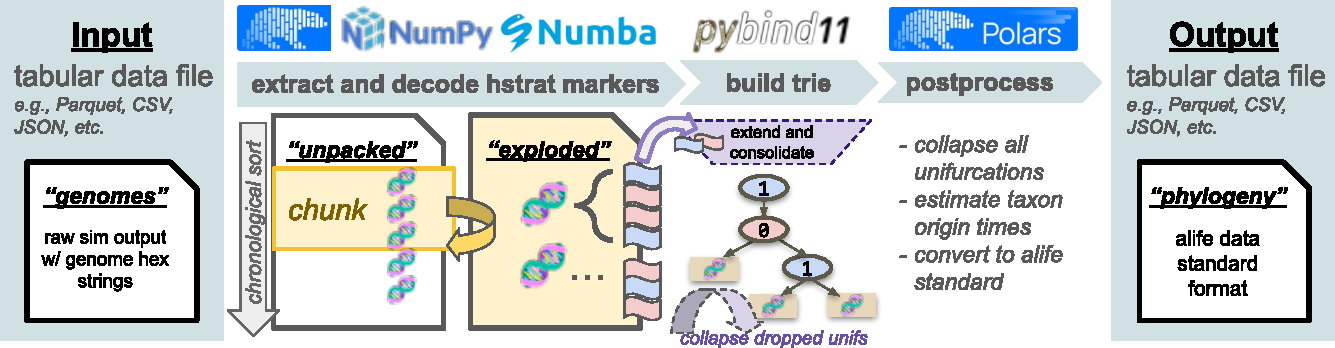
\includegraphics[width=\linewidth]{img/hstratpipeline.pdf}
\caption{\textbf{Schematic of hstrat phylogeny reconstruction pipeline.} TODO.}
\label{fig:hstratpipeline}
\end{figure*}


Supporting software and executable notebooks for this work are available via Zenodo at TODO \citep{moreno2024hsurf}.
DStream algorithm implementations are also published on PyPI in the \texttt{downstream} Python package, where we plan to conduct longer-term, end-user-facing development and maintenance \citep{moreno2024downstream}.
All accompanying materials are provided open-source under the MIT License.

This project benefited significantly from open-source scientific software \citep{2020SciPy-NMeth,harris2020array,reback2020pandas,mckinney-proc-scipy-2010,waskom2021seaborn,hunter2007matplotlib,moreno2023teeplot}.
